%% ============================================================
%% 片段：s05b-amodel   对应原文 PDF 第 117--129 页
%% 本文件由 gw/convert.py 从 arXiv 源码（hep-th/0612073v2）自动生成：
%%   * 公式/编号/引用/图 已经锁定为原文内容，请勿改动任何数学内容与编号；
%%   * 只需把英文正文译为中文，并在每节开头加“本节重点”、关键处加译注。
%% ============================================================


\subsection{\texorpdfstring{$A$-模型}{A-模型}}

%% ==== 原文 §5.3：PDF 第 117 页（印刷第 116 页）====
\label{sec:5.3}

在没有分歧时，$A$-模型中作用于膜上的自然算符是 't Hooft 算符，其定义方式是规定场必须满足的奇点。因此，在有分歧时，我们将寻找类 't Hooft 算符（'t Hooft-like operators）。为简单起见，我们取定义面算符的列维子群（Levi subgroup）为 $\mathbb{L}=\TT$。

要得到 $\Psi=0$，即具有辛结构 $K$ 的 $A$-模型，一个方便的做法是取底层四维理论的扭曲参数（twisting parameter）为 $t=1$，并令四维 $\theta$ 角为零。在一般四维流形 $M$ 上，保持 $A$-模型拓扑对称性的条件已在 \cite{ref8} 的式 (9.1)、(9.2) 中描述。若令 $\CA=A+i\phi$，并记 $\CF=d\CA+\CA\wedge \CA$ 为 $\CA$ 的曲率、$d_A=d+A$，则条件为

% 式 (5.3)
\setcounter{equation}{2}
\begin{equation}\label{eq:5.3}
  \begin{aligned}\CF+i\star \overline\CF & = 0\\
                    d_A\star \phi & = 0.\end{aligned}
\end{equation}


我们具体取 $M=\R\times W$，其中 $\R$ 由“时间”坐标 $s$ 参数化。我们把方程~\eqref{eq:5.3} 限制到与时间无关的情形。其动机在于：通常的 't Hooft 算符由与时间无关的奇点定义（另外也基于 \cite{ref8} 第 9 节引论部分给出的论证，那些论证在有分歧时同样适用）。在与时间无关的情形下，四维联络约化为 $A=A'+A_0\,ds$，其中 $A'$ 是 $G$-丛 $E\to W$ 上的联络，$A_0$ 是取值于 ${\rm ad}(E)$ 的零形式。类似地，写 $\phi=\phi'+\phi_0\,ds$，其中 $\phi'$ 与 $\phi_0$ 是 $W$ 上取值于 ${\rm ad}(E)$ 的形式。令 $\CA'=A'+i\phi'$、$\CF'=d\CA'+\CA'\wedge \CA'$、$\Phi_0=\phi_0-iA_0$。由于此后全部讨论都在三维中进行，我们略去撇号。式~\eqref{eq:5.3} 中的第一个方程变为

% 式 (5.4)
\setcounter{equation}{3}
\begin{equation}\label{eq:5.4}
  \CF=\star\bar {\mathcal D}\Phi_0,
\end{equation}

其中 $\bar{\mathcal D}=d+\bar\CA$，而 $\star$ 此时当然是三维的霍奇 $\star$ 算符。第二个方程变为

% 式 (5.5)
\setcounter{equation}{4}
\begin{equation}\label{eq:5.5}
  D\star \phi={i\over 2}[\bar\Phi_0,\Phi_0].
\end{equation}


\bigskip\noindent{\it 标度对称性}

类 't Hooft 算符用这些方程的奇异解来定义。例如，通常的 't Hooft 算符所用的奇异解在余维三处有奇点，即在孤立点 $r\in W$ 处。该构造在 \cite{ref8} 第 6.2 节中描述过，下面将加以推广。在本文中，我们的主题一直是面算符，它由指定一个余维二奇点——即带有参数 $(\alpha,\beta,\gamma)$ 的熟知奇点——而产生。


% [FIGURE 4] 原文 PDF 第 118 页；caption 见下，需翻译
\begin{figure}[htbp]
  \centering
  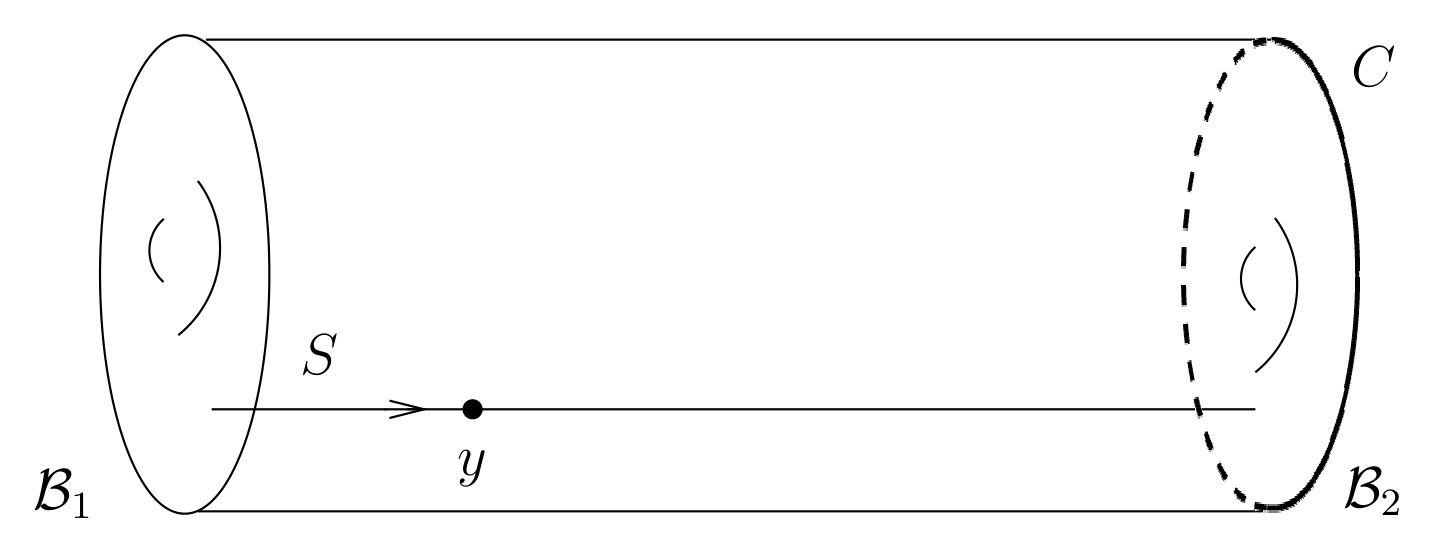
\includegraphics[width=0.62\linewidth]{figures/figure-4.png}
  \caption{支撑在曲面上的线算符，在这一零时刻切片上由直线 $S$ 上的一个点 $y$ 表示。在 $A$-模型中，场沿 $S$ 具有指定的奇点。在 $y$ 附近，奇异行为与 $S$ 上一般点附近的不同。而沿 $S$ 的一般奇异行为，在 $y$ 的两侧又可能不同。（原文 Fig.~4，PDF 第 118 页）}
  \label{fig:4}
\end{figure}

我们感兴趣的是更复杂的情形：一条由余维二奇点构成的曲线 $S$ 含有孤立点 $y$，在该点奇异行为“更糟”。因此，在 $S$ 的一般点附近看到的是通常的余维二奇点，而在点 $y\in S$ 处出现新的奇点。\emph{先验地}，在 $y$ 的左侧，直线 $S$ 由参数 $(\alpha,\beta,\gamma)$ 标记，而在右侧由参数 $(\alpha',\beta',\gamma')$ 标记。若要得到保持 $(B,A,A)$ 型全部超对称的面算符，必须有 $(\beta,\gamma)=(\beta',\gamma')$，因为 $\beta$ 与 $\gamma$ 是 $I$ 型 $B$-模型中的物理参数；要保持该模型的超对称，它们就不能跳变。然而，没有理由只考虑 $\alpha=\alpha'$ 的情形。$(B,A,A)$ 型的拓扑场论局部地与 $\alpha$ 无关，因此应当预期所得到的结果本质上不依赖于 $\alpha$ 与 $\alpha'$。
\begin{yizhu}[易错点]
为什么 $(\beta,\gamma)$ 不能跳而 $\alpha$ 可以跳？根据表~\ref{tab:1} 中复模与 Kähler 模的分配即可看清：$(B,A,A)$ 中唯一的 $B$-模型是 $I$ 型，它只依赖复结构 $I$ 的模 $\beta+i\gamma$，故 $\beta,\gamma$ 是该模型的物理参数，跨过线算符时必须连续；所用的两个 $A$-模型是 $J$ 型与 $K$ 型，它们分别只依赖辛类，而对应的 Kähler 模分别是 $\beta$（在 $J$ 中）与 $\gamma$（在 $K$ 中）。至于 $\alpha$，它在 $I$ 中是 Kähler 模（$I$ 型 $B$-模型不看 Kähler 类），在 $J$ 中是复模 $\gamma+i\alpha$、在 $K$ 中是复模 $\alpha+i\beta$（$A$-模型不看复结构），因此 $\alpha$ 不进入 $(B,A,A)$ 的任何一项，可以在 $y$ 两侧取不同值 $\alpha,\alpha'$。这也正是后文总把 $\beta,\gamma$（以及量子的 $\eta$）与 $\alpha$ 区别对待的原因。
\end{yizhu}

% [FIGURE 5] 原文 PDF 第 119 页；caption 见下，需翻译
\begin{figure}[htbp]
  \centering
  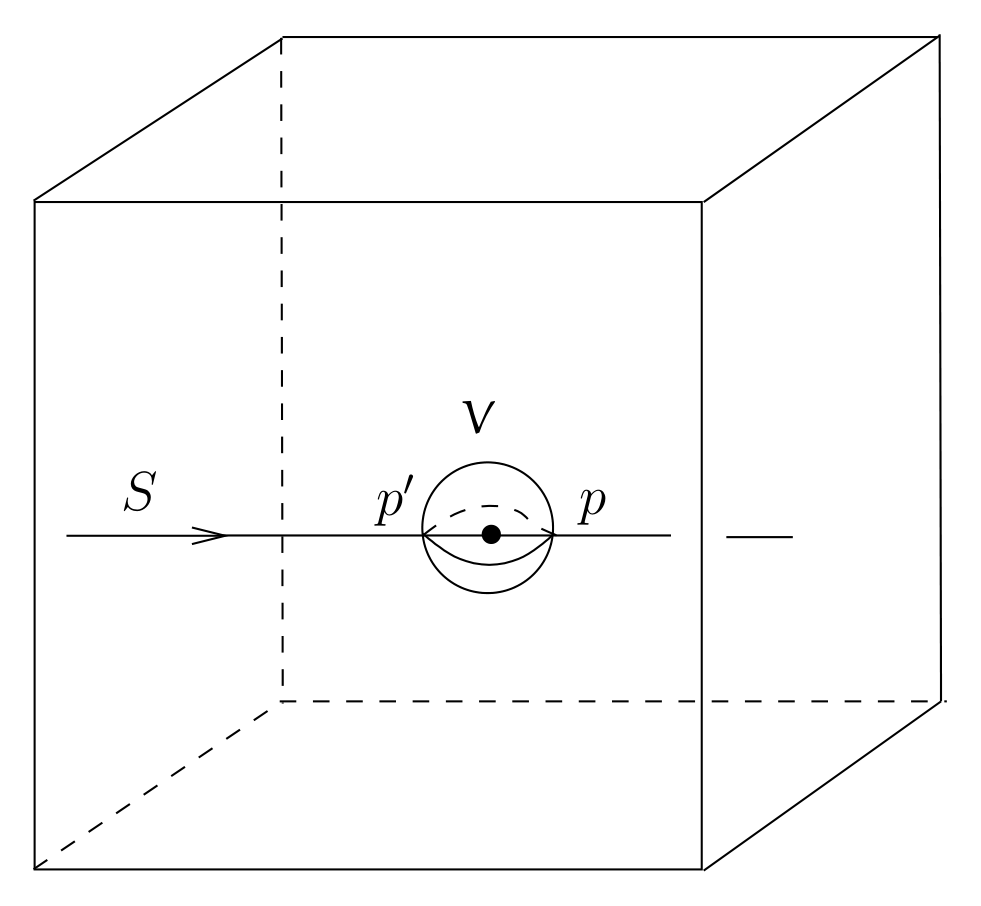
\includegraphics[width=0.62\linewidth]{figures/figure-5.png}
  \caption{为局部地描述该奇点，我们把三维流形 $W$ 换为 $\R^3$，把直线 $S$ 换为 $\R^3$ 中的一条直线 $\R$。点 $y$ 成为 $\R^3$ 的原点，图中以黑点标出。$\EURV$ 是包围原点的单位球面，它与直线 $S$ 交于两点 $p$ 与 $p'$。（原文 Fig.~5，PDF 第 119 页）}
  \label{fig:5}
\end{figure}

为简化，我们对所要寻找的奇点的性质作一假设。假定它们是标度不变的，正如用来定义通常 't Hooft 算符的奇点那样。的确，由于只关心局部的奇异行为，可以把 $W$ 换为 $\R^3$，并以 $y$ 为 $\R^3$ 的原点。在 $\R^3$ 上取欧氏坐标 $x^1,x^2,x^3$，并把图~\ref{fig:5} 中的直线 $S$ 取为 $x^1$ 轴，即由 $x^2=x^3=0$ 定义的那条轴。$\R^3$ 具有标度对称性 $\vec x\to \lambda \vec x$，$\lambda$ 取实正值。所关心的方程在这一标度对称性下不变（若取 $\Phi_0$ 的量纲为 1 来标度），而沿 $S$ 在远离 $y$ 处所需的奇点与标度不变性相容。因此寻找标度不变的奇异解是有意义的，而这已足以满足此处之需。


若从 $\R^3$ 中挖去点 $y$ 再按标度作商，得到 $(\R^3\backslash y)/\R^*_+=S^2\cong \mathbb{CP}^1$。我们称这个商为 $\EURV$。有意思的解大体上可以用 $\EURV$ 上的数据来描述。$\EURV$ 上的场将在图~\ref{fig:5} 所示的两点处奇异，即 $\EURV$ 与直线 $S$ 相交的点 $p$ 与 $p'$。

\bigskip\noindent{\it $\phi=0$ 的情形}

如第~\ref{sec:4.5}~节所述，若 $\beta=\gamma=0$，作用于膜上的算符最为有趣。此时可以取 $\phi=0$（因为 $\phi$ 沿 $S$ 的一般点并无奇点）。结果表明，我们所寻求的类 't Hooft 算符可以用同时满足 $\phi=0$、$A_0=0$ 的奇异解来定义。

这使方程~\eqref{eq:5.4} 与~\eqref{eq:5.5} 大大简化。它们约化为 Bogomolny 方程（Bogomolny equations）

% 式 (5.6)
\setcounter{equation}{5}
\begin{equation}\label{eq:5.6}
  F=\star d_A\Phi_0,
\end{equation}
 其中此时 $F=dA+A\wedge A$、$\Phi_0=\phi_0$ 取值于 $G$ 的实李代数 $\mathfrak g$。我们作一个比标度不变性更强的假设：$A$ 与 $\Phi_0$ 都是从 $\EURV=S^2$ 拉回的。把 $\EURV$ 视为 $\R^3$ 中的单位球面，即由 $r=1$ 定义，其中 $r=|\vec x|$。在 $S^2$ 上得到的方程为
% 式 (5.7)
\setcounter{equation}{6}
\begin{equation}\label{eq:5.7}
  \begin{aligned}F&=-\star\Phi_0\\
                  d_A\Phi_0&=0,\end{aligned}
\end{equation}

                  其中此时这些是二维流形 $\EURV$ 上的方程，$\star$ 取二维意义。例如，为得到第一个方程，我们利用 $\Phi_0$ 对 $r$ 的依赖恰为因子 $1/r$（因 $\Phi_0$ 按权重 1 标度），于是在 $r=1$ 处有 $\partial\Phi_0/\partial r = -\Phi_0$。第二个方程则利用了 $F$ 与 $\partial/\partial r$ 缩并时为零这一事实（因为我们假定解是从 $\EURV$ 拉回的）。

\begin{yizhu}[易错点]
从三维的 $F=\star d_A\Phi_0$ 降到 $\EURV$ 上时，$\star_2\Phi_0$ 前的负号来自 $\star$ 算符的分解而非方程本身：以 $r=|\vec x|$ 为法向，有 $\star_3\omega_2=dr\wedge\star_2\omega_2$ 与 $\star_3(dr\wedge\omega_1)=\star_2\omega_1$；又 $\Phi_0$ 按权重 1 标度，即 $\Phi_0=r^{-1}\Phi_0^{(2)}$，故 $d_A\Phi_0$ 含 $-r^{-1}dr\,\Phi_0^{(2)}$ 一项。代入~\eqref{eq:5.6} 并在 $r=1$ 处分离分量：$dr$ 分量给出 $d_A\Phi_0=0$，纯二维分量给出 $F=-\star_2\Phi_0$。因此~\eqref{eq:5.7} 第一式的负号是 $\star$ 的维数改变带来的，把两式当成同一个方程照抄就会把它丢掉。
\end{yizhu}


显然，两式合起来给出
% 式 (5.8)
\setcounter{equation}{7}
\begin{equation}\label{eq:5.8}
  d_A\star F=0.
\end{equation}

这就是二维杨–米尔斯方程，即由杨–米尔斯作用量导出的欧拉–拉格朗日方程
% 式 (5.9)
\setcounter{equation}{8}
\begin{equation}\label{eq:5.9}
  {\bm{I}}=-{1\over
2}\int_\EURV\,\,\Tr \,F\wedge \star F.
\end{equation}


这些方程还有如下解释。给定黎曼面 $\EURV$，$G$-丛 $E\to
\EURV$ 上的每个联络 $A$ 都赋予 $E$ 一个全纯结构，它由 $\bar\partial$ 算符 $\bar \partial_A=d\bar z(\partial_{\bar z}+A_{\bar
z})$ 定义。反过来，也可以从全纯
$G_\C$-丛 $E\to \EURV$ 出发，问 $E$ 容许哪些与其全纯结构相容的酉联络（相容是指由该联络诱导的全纯结构与 $E$ 给定的全纯结构一致）。稳定与半稳定丛正是那些容许与其全纯结构相容的平坦酉联络的丛 \cite{ref51}。更一般地，若给 $\EURV$ 配上 Kähler 度量从而有 $\star$ 算符（使得杨–米尔斯方程与作用量有定义），则据 \cite{ref52}，每个 $G_\C$-丛 $E\to \EURV$（无论稳定与否）都容许一个酉联络，它在规范变换下唯一，满足杨–米尔斯方程并与 $E$ 的全纯结构相容。于是特别地，模去规范变换的杨–米尔斯方程解，与全纯 $G_\C$-丛的等价类自然对应。

这一结果在杨–米尔斯作用量的梯度流（gradient flow）\cite{ref52} 中有自然的解释，但此处不需要。对我们更重要的是把上述结果推广到容许抛物结构的情形 \cite{ref77}。我们将对任意数目的分歧点、任意选取的抛物子群陈述这一定理。从黎曼面 $\EURV$ 中挖去有限个点 $p_1,\dots,p_s$。给每个 $p_i$ 标上一个抛物权（parabolic weight）$\alpha_i \in \mathfrak t$，以及相联系的共轭类 $U_i=\exp(-2\pi\alpha_i)$。假定 $\alpha_i$ 足够一般，使得对每个 $i$，与 $\alpha_i$ 交换的列维子群 $\mathbb{L}_i\subset G$ 与和 $U_i$ 交换的子群相同；记 ${\EUP}_i$ 为由配对 $(\mathbb{L},\alpha_i)$ 决定的抛物子群。考虑 $G$-丛 $E\to \EURV\backslash
\{p_1,\dots,p_s\}$ 上满足杨–米尔斯方程的联络 $A$，它绕点 $p_i$ 的和乐与 $U_i$ 共轭。该断言是：这样的联络（模去规范变换）与在点 $p_i$ 处具有（$\EUP_i$ 型）抛物结构的全纯 $G_\C$-丛 $E\to \EURV$ 一一对应。抛物丛稳定或半稳定，当且仅当对应的杨–米尔斯方程解是平坦的；否则它是不稳定的。
\begin{yizhu}[含糊点拨]
作者把“Bogomolny 方程 $\to$ 二维杨–米尔斯方程 $\to$ 全纯丛／抛物丛”这条链当作已知结果引用（\cite{ref51,ref52,ref77}），其中被略去的论证是：二维杨–米尔斯方程 $F=-\star\Phi_0$、$d_A\Phi_0=0$ 合起来即 $d_A\star F=0$，也就是曲率（等价地 $\star F$）协变常；在紧黎曼面上，满足杨–米尔斯方程的酉联络模去规范变换，恰好给出全纯 $G_\C$-丛的模空间（Narasimhan–Seshadri 定理的微分几何形式），稳定／半稳定丛对应解的存在性；带抛物结构时（Mehta–Seshadri、Biquard 等的定理 \cite{ref77}），对应的解析对象是带抛物权与抛物型约化的全纯丛，平坦解对应稳定抛物丛。正是这一定理链条，使我们可以用 $\mathbb{CP}^1$ 上两点处的抛物丛来分类类 't Hooft 算符。
\end{yizhu}

在应用这一定理时，由于我们取面算符为 $\TT$ 型，眼下关心的是各 $\mathbb{L}_i$ 都与极大环面 $\TT$ 共轭的情形。因此，在本节末尾简要讨论一般 $\mathbb{L}$ 型面算符之前，“抛物结构”一词都指把结构群约化到博雷尔子群（Borel subgroup）$\EUB$。

\bigskip\noindent{\it $SL(2,\C)$ 的抛物丛}

为构造类 't Hooft 算符，我们关心 $\EURV=\mathbb{CP}^1$ 上在两点 $p$ 与 $p'$ 处具有抛物结构的 $G_\C$-丛。这两点处的抛物权为 $\alpha$ 与 $-\alpha'$。出现负号的原因是：在图~\ref{fig:5} 中，二维球面 $\EURV$ 与直线 $S$ 在点 $p$ 与 $p'$ 处以相反的定向相交。
\begin{yizhu}[易错点]
图~\ref{fig:5} 的几何是理解两个点（puncture）$p$、$p'$ 的关键：$\EURV$ 是 $\R^3$ 中以原点（即点 $y$）为中心的单位球面，直线 $S$（$x^1$ 轴）穿过球心，故与 $\EURV$ 交于两点 $p$、$p'$，二者互为对径点（图中 $p'$ 在左、$p$ 在右，箭头给出 $S$ 的定向）。$S$ 的定向在穿过球心的两侧相对球面给出相反的指向，于是在 $p$ 与 $p'$ 处测得的奇异参数相差一个符号，抛物权写作 $\alpha$ 与 $-\alpha'$；若算符两侧参数不跳（$\alpha=\alpha'$），两点处的权就是 $\alpha$ 与 $-\alpha$。这也解释了单值性公式 $U=\exp(-2\pi\epsilon\alpha)$、$U'=\exp(2\pi\epsilon'\alpha')$ 中 $\epsilon'$ 带来的符号自由度。
\end{yizhu}

这种情形下的抛物丛可以非常具体地描述。为说明关键思想，取 $G_\C=SL(2,\C)$，并同时从全纯的观点和利用与杨–米尔斯方程的关系来进行分析。

从全纯观点看，$SL(2,\C)$ 丛 $E\to \EURV$（视为行列式平凡、秩为 2 的向量丛）必为 $\CO(m)\oplus \CO(-m)$，其中 $m$ 为某整数，不妨假定它非负。此外，还必须在两点 $p,p'\in
\EURV$ 处给 $E$ 配上抛物结构。对黎曼面上给定点处的秩 2 丛 $E$，抛物结构不过是在该点处 $E$ 的纤维中选取一个一维子空间。记这两处的纤维为 $E|_p$ 与 $E|_{p'}$。于是点 $p$ 与 $p'$ 处的抛物结构由子空间 $E_p\subset E|_p$ 与 $E_{p'}\subset E|_{p'}$ 的选取给出。这类抛物丛的同构类可如下分类：

(1) 先设 $m=0$。此时丛 $E$ 平凡，群 $G_\C\cong
SL(2,\C)$ 作用于其上。若 $E$ 存在一个非零整体截面，其到 $p$ 的限制取值于 $E_p$、到 $p'$ 的限制取值于 $E_{p'}$，我们就说 $p$ 与 $p'$ 处的抛物结构一致。否则说它们不一致。在同构意义下，即模去 $SL(2,\C)$ 的作用，恰有两种选择：$p$ 与 $p'$ 处的抛物结构或者一致，或者不一致。

(2) 现在设 $m>0$。丛 $E=\CO(m)\oplus \CO(-m)$ 有唯一的子丛同构于 $\CO(m)$（其特征是：$E$ 的任意整体全纯截面实际上都是这个子丛的截面）。相比之下，$\CO(-m)$ 在 $E$ 中的嵌入、从而分裂 $E=\CO(m)\oplus \CO(-m)$ 并非典范的。模去 $E$ 的自同构，抛物结构中唯一的不变量信息是：子空间 $E_p$ 与 $E_{p'}$ 是否与 $\CO(m)$ 在 $p$ 与 $p'$ 处的纤维重合。因此对给定的 $m$，共有 $2\times 2=4$ 种选择。我们把这四种可能组织如下。若 $E_p=\CO(m)|_p$，就用整数 $m$ 标记抛物丛 $E$；否则用 $-m$ 标记它。并且，若 $E_p$ 与 $E_{p'}$ 或者都与 $\CO(m)$ 的相关纤维重合、或者都与它不同，我们就说 $p'$ 处的抛物结构与 $p$ 处的一致。否则说抛物结构不一致。

现在从杨–米尔斯方程的观点来看。此时需要在点 $p$ 与 $p'$ 处选取抛物权。（这些权没有进入全纯描述，因为我们并不关心哪些抛物丛稳定。）取

% 式 (5.10)
\setcounter{equation}{9}
\begin{equation}\label{eq:5.10}
  \begin{aligned}\alpha&=iy\,\left(\begin{matrix}1 & 0\\ 0&-1\end{matrix}\right)\\
\alpha'&=iy'\,\left(\begin{matrix}1 & 0\\ 0&-1\end{matrix}\right),\end{aligned}
\end{equation}

其中 $0<y,y'<1/2$。初始时取 $y\not=y'$ 也较为方便。

杨–米尔斯方程~\eqref{eq:5.8} 表明曲率是协变常的，因此可以选取一个规范使曲率实际上是常数
% 式 (5.11)
\setcounter{equation}{10}
\begin{equation}\label{eq:5.11}
  F=i\left(\begin{matrix}f & 0\\ 0 &
-f\end{matrix}\right),
\end{equation}
 其中 $f$ 为实常数，不妨取非负。稍后就会看到，若 $y\not=
y'$ 则 $f\not=0$。由于 $F$ 协变常，它与绕点 $p$ 与 $p'$ 的和乐 $U$、$U'$ 交换，因此（假定 $f\not=0$）这些和乐是对角矩阵。由于和乐必须分别与 $\exp(-2\pi\alpha)$ 和 $\exp(-2\pi (-\alpha'))$ 共轭，于是 $U=\exp(- 2\pi\epsilon \alpha)$、$U'=\exp(2\pi\epsilon'\alpha')$，其中 $\epsilon,\epsilon'=\pm 1$。

最后，具有上述联络与曲率的丛 $E$ 存在，当且仅当

% 式 (5.12)
\setcounter{equation}{11}
\begin{equation}\label{eq:5.12}
  \exp\left(\int_{\EURV}F\right)=UU'.
\end{equation}
 该条件等价于
% 式 (5.13)
\setcounter{equation}{12}
\begin{equation}\label{eq:5.13}
  \int_\EURV{f\over 2\pi}+\epsilon
y-\epsilon' y'= m',
\end{equation}
 其中 $m'$ 为某整数。

\begin{yizhu}[物理图像补充]
式~\eqref{eq:5.12} 是 Stokes 定理在 $\EURV$ 上的体现：绕 $p$ 与 $p'$ 的两个小圈之和与绕整个 $\EURV$ 的大圈同调，故绕大圈的和乐 $\exp(\int_{\EURV}F)$ 等于两个小圈的和乐之积 $UU'$（不计一次共轭，视基点而定）。把它对角化即得~\eqref{eq:5.13}：$\int_{\EURV}f/2\pi+\epsilon y-\epsilon'y'=m'\in\Z$，其中 $m'$ 是本征值所对应的整数，$\epsilon,\epsilon'$ 是 $\alpha$ 与 $-\alpha'$ 的权同 $\pm y$ 的配对符号。给定 $y,y'$ 与 $\epsilon,\epsilon'$ 后，整数 $m'$ 唯一决定 $\int_{\EURV}f/2\pi\ge 0$，即决定曲率的大小。
\end{yizhu}

外尔群通过改变 $F$、$y$、$y'$ 与 $m'$ 的符号来作用。因此，经一个外尔变换可固定 $\epsilon=1$；此后杨–米尔斯方程的解由整数 $m'$ 与变量 $\epsilon'\in\{\pm 1\}$ 标记。我们所给出的杨–米尔斯方程解的分类在 $y=y'$ 时同样成立，但此时处理 $\epsilon'=1$、$m'=0$ 的情形需要稍加小心。

\begin{yizhu}[含糊点拨]
「稍加小心」指的是 $f=0$ 这一支。~\eqref{eq:5.13} 中 $f\ge 0$，故 $f=0$ 当且仅当 $m'=\epsilon y-\epsilon'y'$；而 $0<y,y'<1/2$ 使 $\epsilon y-\epsilon'y'\in(-1,1)$，又必须是整数，于是 $f=0$ 只发生在 $y=y'$、$\epsilon=\epsilon'$、$m'=0$ 时。此时 $U'=\exp(2\pi\epsilon'\alpha')=\exp(2\pi\alpha)=U^{-1}$，故 $UU'=1$，与~\eqref{eq:5.12} 相容；反过来若固定 $\epsilon=1$ 而取 $\epsilon'=-1$（仍 $y=y'$），则 $U'=U$、$UU'=\exp(-4\pi\alpha)\ne 1$，与~\eqref{eq:5.12} 矛盾，该支并不存在。上文「假定 $f\ne 0$ 故和乐为对角矩阵」的论证在 $f=0$ 时确实失效。
\end{yizhu}

于是，杨–米尔斯解的分类与抛物丛的分类一致。在这一比较中，$m'$ 对应于 $m$，而 $\epsilon'=1$（或 $-1$）对应于两处抛物结构一致（或不一致）的情形。

每个这样的解或丛都使我们能够定义一个类 't Hooft 算符。于是，对每一对 $(m,\epsilon')\in \Z\times \Z_2$ 都得到一个类 't Hooft 算符 $T_{m,\epsilon'}$。

这些算符确实保持 $(B,A,A)$ 型的全部拓扑超对称。为看出这一点，首先注意：由于它们来自所需方程~\eqref{eq:5.4} 与~\eqref{eq:5.5} 的解，它们保持 $K$ 型 $A$-模型（具有辛结构 $\omega_K$ 的那个）的拓扑对称性。由于这些解在 $\varphi\to i\varphi$ 下不变，而该变换把辛结构 $\omega_K$ 旋转为 $\omega_J$，它们也保持 $J$ 型 $A$-模型的拓扑对称性。这两个超荷的线性组合生成 $(B,A,A)$ 型的全部拓扑超对称。
\begin{yizhu}[易错点]
$(B,A,A)$ 型超对称的含义是：在复结构 $I$ 上取 $B$-模型，在复结构 $J$ 与 $K$ 上取 $A$-模型。本节从 $\Psi=0$ 出发：按第~\ref{sec:5}~节，$\Psi=0$ 一侧的拓扑场论是 $\MH$ 上辛结构 $\omega_K$ 的 $A$-模型（而另一端点 $\Psi=\infty$ 给出复结构 $J$ 上的 $B$-模型）。$A$-模型只依赖辛结构（复化 Kähler 类）而与复结构无关，于是本段的论证分两步：解来自~\eqref{eq:5.4}、\eqref{eq:5.5}，故保持 $K$ 型 $A$-模型的拓扑对称性；解又在 $\varphi\to i\varphi$ 下不变，而该操作把 $\omega_K$ 旋转为 $\omega_J$，故也保持 $J$ 型 $A$-模型的拓扑对称性；两个超荷的线性组合即生成完整的 $(B,A,A)$。易错之处：$\varphi\to i\varphi$ 并非解的对称性，而是把 $K$ 型解映为同形式的 $J$ 型解（后文纳入 $\beta,\gamma$ 时还会用到这一点）。
\end{yizhu}


\bigskip\noindent{\it 在膜上的作用}


% [FIGURE 6] 原文 PDF 第 124 页；caption 见下，需翻译
\begin{figure}[htbp]
  \centering
  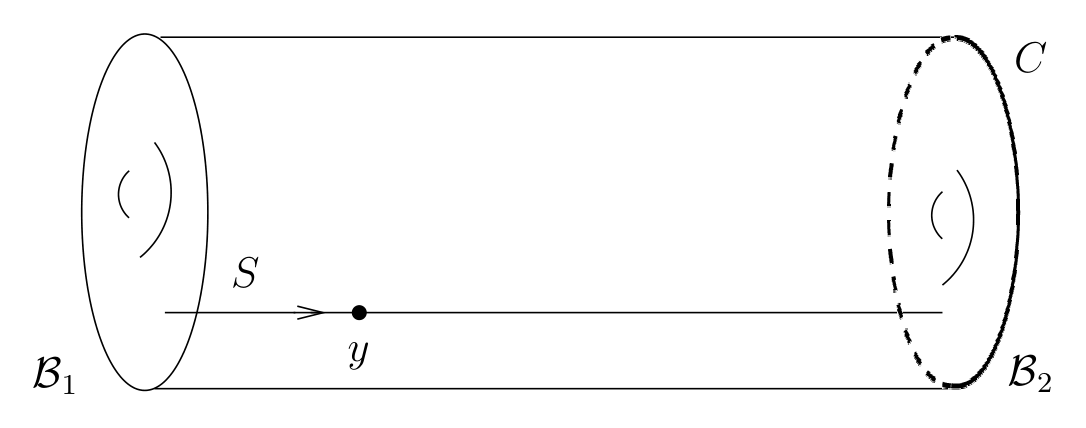
\includegraphics[width=0.62\linewidth]{figures/figure-6.png}
  \caption{线算符（此处插入在点 $y$）在膜上的作用。场 $(A,\phi)$ 对每个 $u\in S$ 都在复结构 $I$ 中确定一个带分歧的希格斯丛 $E_u\to C_u=\{u\}\times C$。在超对称方程的解中，$E_u$ 的全纯类型为常数，除非 $C_u$ 越过点 $y$——越过时它发生跳变。（原文 Fig.~6，PDF 第 124 页）}
  \label{fig:6}
\end{figure}

粗略地说，这些类 't Hooft 算符之一在膜上的作用，类似于无分歧情形中通常 't Hooft 算符的作用，如 \cite{ref8} 所述。因此我们只作相当简略的说明。


在图~\ref{fig:6} 中，我们考虑三维流形 $W=I\times C$ 上 $G$-丛 $E$ 的场 $(A,\phi)$，它们沿直线 $S$ 具有通常的奇点。对任意 $u\in I$，把丛 $E$ 与场 $A,\phi$ 限制到 $C_u=\{u\}\times C$，得到带分歧的希格斯丛 $E_u\to C_u$。若满足 Bogomolny 方程~\eqref{eq:5.6}，则 $E_u$ 的全纯类型与 $u$ 无关，除非越过某个线算符所在的位置。若越过的是支撑在 $C$ 中一般点（乘 $I$ 中一点）处的线算符，则丛 $E_u$ 经历通常的 Hecke 修改；而若如图~\ref{fig:6} 那样越过支撑在 $S$ 上的线算符，则得到更一般的类 Hecke 修改，它可以涉及抛物结构。这些陈述的理由与 \cite{ref8} 中相同。

现在设我们想看出图~\ref{fig:6} 中点 $y$ 处的线算符 $L_y$ 如何作用在，比如说，图左侧的膜 ${\mathcal B}_1$ 上。刚才所述意味着算符 $L_y$ 确定一个“对应”${\EUQ}\subset \MH\times \MH$。$\EUQ$ 参数化对 $(\tilde E_u,E_u)$，其中 $\tilde E_u$ 可由 $E_u$ 通过“跳过”线算符 $L_y$ 得到。$\EUQ$ 可视为 $\MH\times \MH$ 中 $(B,A,A)$ 型的膜，因为它由保持该对称性的方程之解得到。我们主要把它看作 $K$ 型的 $A$-膜。

事实上，可用来定义类 't Hooft 算符 $L_y$ 的 $\EURV\cong \mathbb{CP}^1$ 上的抛物丛大多是不稳定的。出现这种情况时，我们实际上希望用配对 $(\tilde E_u, E_u)$ 的空间作紧化来定义 $\EUQ$，即把用不那么不稳定的抛物丛（对 $G_\C=SL(2,\C)$ 来说就是 $|m|$ 更小）所定义的类 Hecke 修改也包括进去。这与无分歧情形完全类似。可以预期，原则上这种紧化的使用能由底层的四维规范场论来论证。

现设 $\pi_i$（$i=1,2$）为两个投影 $\pi_i:\MH\times\MH\to \MH$。给定 $\MH$ 上的膜 ${\mathcal B}_1$，我们把它经 $\pi_1^*$“拉回”到 $\MH\times \MH$，与 $\EUQ$ 作张量积，再经 $p_{2}$“前推”到 $\MH$，得到新的膜 $L_y\cdot {\mathcal B}_1$。即 $L_y\cdot {\mathcal B}_1=\pi_{2\,*}(p_1^*({\mathcal B}_1)\otimes
\EUQ)$。若 ${\mathcal B}_1$ 是 $(B,A,A)$ 型的膜，这些运算可以用复结构 $I$ 中的复几何来实施；但更一般地，若 ${\mathcal B}_1$ 只是 $K$ 型的 $A$-膜，则必须使用这些运算在 $A$-模型中的类比，即在 Floer 上同调中的类比。
\begin{yizhu}[原文疑误]
原文此处（PDF 第 125 页）刚把两个投影定义为 $\pi_1,\pi_2$，紧接着却说经 $p_2$“前推”，并在同一公式中写出 $p_1^*$，同时又用 $\pi_{2\,*}$；由上下文看 $p_1,p_2$ 与 $\pi_1,\pi_2$ 指同一对投影，应是原文的记号笔误。译文照原文保留 $p_1,p_2$，不作改动。另：图~\ref{fig:6} 的 caption 写作“对每个 $u\in S$”，而正文为“对任意 $u\in I$”——$S$ 是 $W=I\times C$ 中沿时间方向的直线，两者可理解为把 $u$ 记作沿 $S$ 的时间参数；译文亦照原文保留。
\end{yizhu}


下面给出一个或许更朴素的解释。为构造图~\ref{fig:6} 情形下的物理希尔伯特空间（两端由膜给出边界条件、内部有算符 $L_y$），可如下进行。考虑超对称位形的紧化模空间 $\bar{\mathcal N}$，其边界条件由两端的膜 ${\mathcal B}_1$、${\mathcal B}_2$ 以及内部的 $L_y$ 确定。物理希尔伯特空间是 $\bar{\mathcal N}$ 的上同调。为定义 $L_y$ 在膜上的作用，其想法是：$\bar{\mathcal N}$ 的上同调，与去掉 $L_y$ 造成的奇点、并把 ${\mathcal B}_1$ 换为另一个膜 $L_y\cdot{\mathcal B}_1$（它将不依赖于 ${\mathcal B}_2$）之后所得到的上同调相同。$L_y\cdot{\mathcal B}_1$ 的 Chan–Paton 层（Chan-Paton sheaf）在点 $E_u\in\MH$ 处的纤维，等于按如下方式得到的空间 $\Xi(E_u)$ 的上同调：$\Xi(E_u)$ 参数化希格斯丛 $\tilde E_u$，使得对 $(\tilde E_u,E_u)$ 代表 $\EUQ$ 中的一个点。（在这个过分简化的解释中，我们忽略了 $\EUQ$ 的奇点。）只要仔细考虑有、无算符 $L_y$ 插入时物理希尔伯特空间如何计算，就可以为这一方案提供论证。

\begin{yizhu}[物理图像补充]
公式 $\pi_{2,*}(\pi_1^*(\mathcal B_1)\otimes\EUQ)$ 就是由核 $\EUQ$ 给出的积分变换。在 $I$ 型 $B$-模型里，$\mathcal B_1$ 是 $\MH$ 上的相干层复形，$\otimes$ 取导出张量积、$\pi_{2,*}$ 取导出推前，这正是 Fourier--Mukai 型函子；而导出推前在点 $E_u$ 处的纤维恰为 $R\Gamma(\Xi(E_u),\cdot)$，其全上同调即文中说的「$\Xi(E_u)$ 的上同调」。换到 $K$ 型的 $A$-模型，$\MH$ 的辛结构使膜成为 $\omega_K$-拉格朗日膜，$\EUQ$ 成为拉格朗日对应，$\otimes$ 换成纤维积、$\pi_*$ 换成 Floer 复形，这就是段末所说「在 Floer 上同调中的类比」。
\end{yizhu}


\bigskip\noindent{\it 仿射外尔群与辫群}

现在回到 $G_\C=SL(2,\C)$ 的例子，其中我们把类 't Hooft 算符按对 $(m,\epsilon')\in \Z\times\Z_2$ 作了分类。$SL(2,\C)$ 的仿射外尔群 $\AffWeyl$（已在式~\eqref{eq:3.50} 中引入）是一个扩张
% 式 (5.14)
\setcounter{equation}{13}
\begin{equation}\label{eq:5.14}
  0\to \Z\to \AffWeyl\to\Z_2\to 0,
\end{equation}
 而该群的元素相当自然地由配对 $(m,\epsilon')$ 标记，正如类 't Hooft 算符那样。实际上，由于 $\Z_2$ 通过变号作用于 $\Z$，$m$ 的符号有一点微妙之处，正如 't Hooft 算符那里的情形一样。't Hooft 算符与 $\AffWeyl$ 的元素之间的对应，比二者中任何一个与配对 $(m,\epsilon')$ 的对应都更自然。

\begin{yizhu}[物理图像补充]
对 $G=SL(2,\C)$，式~\eqref{eq:5.14} 就是无限二面体群的正合列：由~\eqref{eq:3.50}，$\AffWeyl=\Lambda_{\rm cort}\rtimes\Weyl$，此处 $\Lambda_{\rm cort}\cong\Z$、$\Weyl=\Z_2$，故 $\AffWeyl\cong\Z\rtimes\Z_2$。$\Z_2$ 的生成元把平移 $m$ 共轭为 $-m$，这正是文中「$m$ 的符号有一点微妙之处」的来源：$(m,\epsilon')$ 与 $(-m,\epsilon')$ 是两个不同的群元素，须先选定 $\epsilon'$ 的代表元，标号才唯一；也正因如此，算符与 $\AffWeyl$ 的元素之间的对应，比它与 $(m,\epsilon')$ 的对应更自然。
\end{yizhu}

对任意单连通的 $G$ 有类似的结论：$\mathbb{CP}^1$ 上恰在两点处具有抛物结构的丛，自然地对应于 $\AffWeyl$ 的元素。这在杨–米尔斯进路中相当容易看出：把我们对 $SL(2,\C)$ 给出的论证加以推广即可，故留作练习。这在全纯进路中也是一个标准结果。\footnote{它等价于如下陈述：$\mathbb{CP}^1$ 上在两点处具有抛物结构的丛，对应于 Iwahori 群在仿射旗流形上作用的轨道。}



% [FIGURE 7] 原文 PDF 第 127 页；caption 见下，需翻译
\begin{figure}[htbp]
  \centering
  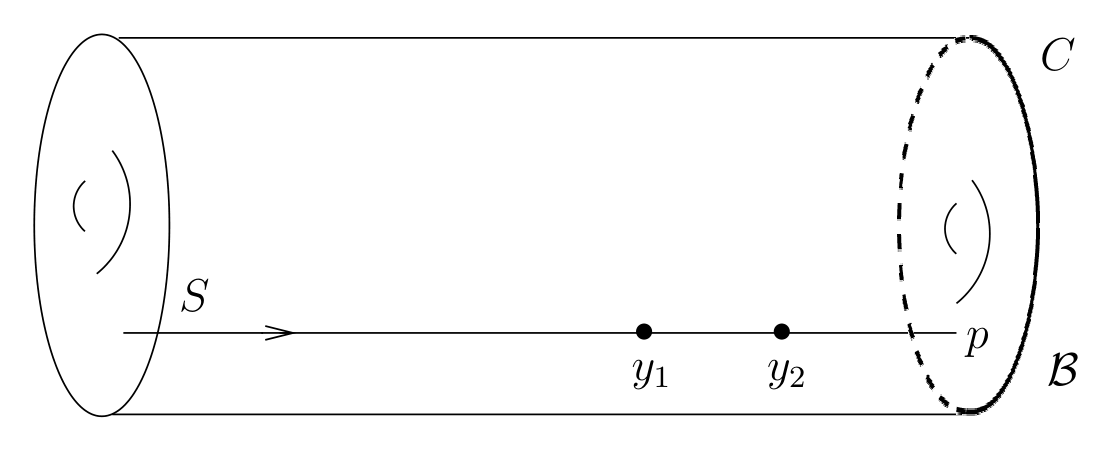
\includegraphics[width=0.62\linewidth]{figures/figure-7.png}
  \caption{共存于某个面算符的支撑上的两个线算符，可以通过简单地把两条线移到一起而复合。在此描绘的静态情形中，这通过取 $y_1\to y_2$ 的极限来实现。在拓扑场论中，线算符生成一个作用于膜的结合代数。（原文 Fig.~7，PDF 第 127 页）}
  \label{fig:7}
\end{figure}

我们所定义的类 't Hooft 算符可以通过把两条线移到一起而以自然方式复合，如图~\ref{fig:7} 所示。或许会预期这些算符按仿射外尔群的乘法法则复合。然而，据 \cite{ref29} 以及我们在第~\ref{sec:4.5}~节中的论证，应当预期：在分歧点 $p\in C$ 处作用于 $A$-模型之膜的群是仿射辫群（affine braid group），而不是仿射外尔群。如式~\eqref{eq:4.16} 那样，两个群由一个正合列相联系
% 式 (5.15)
\setcounter{equation}{14}
\begin{equation}\label{eq:5.15}
  1\to
\pi_1(\eurz)\to B_{\rm aff}\to \AffWeyl\to 1,
\end{equation}
 其中 $\eurz$ 是 $\AffWeyl$ 自由作用的空间，由配对 $(\alpha,\beta)\in \mathfrak t\times \mathfrak t$ 构成。这是一个非平凡扩张，因此 $\AffWeyl$ 可以提升到 $B_{\rm aff}$，但这样的提升不保持群运算。因此，我们不预期作用于膜上的算符 $T_{m,\epsilon'}$ 尊重仿射外尔群的这些关系。

\begin{yizhu}[易错点]
式~\eqref{eq:5.15} 的 $\AffWeyl$、$B_{\rm aff}$ 没有标注 ${}^L$，而第~\ref{sec:4.5}~节的式~\eqref{eq:4.16} 明写作 $B_{\rm aff}({}^L\neg G)$、$\AffWeyl({}^L\neg G)$；第~4.5~节那里讨论 $Y=1$ 的情形，$\eurq_Y$ 是 $\bar\TT_\C$ 的正则点、其商是 $\bar G_\C$ 的正则共轭类空间，所得的群按定义就是 ${}^L\!G$ 的仿射辫群（该节译注已指出该处 ${}^L$ 标注与邻近约定略有出入）。两处 $\eurz$ 其实是同一个空间，即 $\AffWeyl$ 自由作用的正则序对 $(\alpha,\beta)\in\mathfrak t\times\mathfrak t$；本节讨论 $\mathbb{CP}^1$ 上两点的抛物 $G_\C$-丛与 't Hooft 算符，故按 $G$ 标号。两列形式相同而群不同，不可混用；译文照原文保留。
\end{yizhu}

可以稍微具体一些。对秩为 $r$ 的 $G$，$\AffWeyl$ 由基本反射 $T_i$（$i=1,\dots,r+1$）生成，Dynkin 图的每个节点对应一个。它们满足 $T_i^2=1$ 以及某些附加关系。例如，对秩大于 1 的单边型（simply-laced）$G$，若顶点 $i$ 与 $j$ 由一条边相连，则

% 式 (5.16)
\setcounter{equation}{15}
\begin{equation}\label{eq:5.16}
  T_iT_jT_i=T_jT_iT_j
\end{equation}

若不相连，则

% 式 (5.17)
\setcounter{equation}{16}
\begin{equation}\label{eq:5.17}
  T_iT_j=T_jT_i
\end{equation}

要得到仿射辫群，只需去掉关系 $T_i^2=1$，保留其余关系。仿射外尔群中长度最短的词，可以相当自然地提升为仿射辫群中的“同一个”词，但这并不给出群同态。

\begin{yizhu}[含糊点拨]
「不能给出同态」的精确含义是~\eqref{eq:5.15} 作为群扩张不可裂：若存在同态 $s:\AffWeyl\to B_{\rm aff}$ 使 $B_{\rm aff}\to\AffWeyl$ 与之合成为恒等，则 $\AffWeyl$ 的每个关系在 $B_{\rm aff}$ 中都成立，特别地 $T_i^2=1$ 成立；但仿射辫群恰恰是删去 $T_i^2=1$、保留~\eqref{eq:5.16} 与~\eqref{eq:5.17} 得到的，其中 $T_i^2\ne 1$。故原文的「非平凡扩张」应读作「不分裂」：最短词给出的是集合论截面，只保证辫关系成立，不保证群运算，这正是「不预期算符 $T_{m,\epsilon'}$ 尊重仿射外尔群的关系」的意思。
\end{yizhu}


这里我们不试图用规范场论方法描述对应于 $\pi_1(\eurz)$ 的在膜上的运算。在例子中，$\pi_1(\eurz)$ 似乎通过把膜的 Chan–Paton 丛与某些具有非平凡鬼数（ghost number）作用的向量丛作张量积来作用。

\begin{yizhu}[易错点]
两套 $T$ 记号不要混：$T_i$（$i=1,\dots,r+1$）是仿射 Dynkin 图节点所对应的基本反射，$T_{m,\epsilon'}$ 则是按 $\AffWeyl$ 的元素（由配对 $(m,\epsilon')$ 标号）命名的类 't Hooft 算符。生成元有 $r+1$ 个而非 $r$ 个；对 $G=SL(2,\C)$（$r=1$）只有 $T_1,T_2$，而 $\widehat{A_1}$ 的图是双边，不属于文中「秩大于 1 的单边型」，故~\eqref{eq:5.16} 不适用于此例：此时 $\AffWeyl\cong\Z\rtimes\Z_2$，除 $T_i^2=1$ 外并无辫关系，式~\eqref{eq:5.16} 只是单边型情形才有的「附加关系」。
\end{yizhu}



\bigskip\noindent{\it $\beta$ 与 $\gamma$ 的纳入}

到目前为止我们都取希格斯场 $\phi$ 为零，而这只有在 $\beta=\gamma=0$ 时才有意义。若 $(\beta,\gamma)\not=0$，则 $\phi$ 具有指定的奇点，不能为零。

把 $\beta$ 与 $\gamma$ 纳入分析出乎意料地直接，理由如下。我们用来描述算符 $T_{m,\epsilon'}$ 的杨–米尔斯方程解实际上全是阿贝尔的，即结构群从 $G$ 约化到其极大环面 $\TT$。这反映了挖去两点的二维球面的基本群是阿贝尔群这一事实。

既然如此，只需为 $\phi$ 显式地加上一个阿贝尔解，就能把 $\beta$ 与 $\gamma$ 纳入。给定 $(\beta,\gamma)\in \mathfrak t$，定义

% 式 (5.18)
\setcounter{equation}{17}
\begin{equation}\label{eq:5.18}
  \varphi =\half(\beta+i\gamma){dz\over z},
\end{equation}
 其中 $z=x^2+ix^3$，$x^2$ 与 $x^3$ 是直线 $S\subset W=\R^3$ 的法坐标。（$\varphi$ 不是从 $\EURV$ 拉回的。）于是令 $\phi=\varphi+\bar\varphi$（仍取 $A_0=0$），即满足方程~\eqref{eq:5.4} 与~\eqref{eq:5.5}。$\varphi$ 的奇点与 $x^1$ 无关；因此正如所预期的，这一构造只有在 $\beta$ 与 $\gamma$（不同于 $\alpha$）越过线算符的支撑时不跳变的前提下才可能。

\begin{yizhu}[物理图像补充]
能把 $A$ 与 $\varphi$ 直接叠加，靠的是解的阿贝尔性：'t Hooft 解中的 $A$、$\Phi_0$ 与这里的 $\beta,\gamma$ 都取值于 $\mathfrak t$，而 $[\mathfrak t,\mathfrak t]=0$，故 $\phi\wedge\phi=\sum_{a,b}\phi^a\wedge\phi^b[T_a,T_b]=0$、$[A,\phi]=0$、$[\bar\CA,\Phi_0]=0$，于是 $\CF$ 与 $\bar{\mathcal D}\Phi_0$ 都不因加上 $\varphi$ 而改变；又 $z\ne 0$ 时 $d\varphi=0$，故 $\phi=\varphi+\bar\varphi$ 自动满足~\eqref{eq:5.5}。若换成非阿贝尔解，$\CF$ 会多出 $-\phi\wedge\phi+i d_A\phi$，这一叠加就不成立，文中强调「阿贝尔解」正在于此。
\end{yizhu}

如此得到的线算符确实保持 $(B,A,A)$ 型的拓扑对称性。在移植我们在 $\varphi=0$ 处给出的论证时，只需注意一处。变换 $\varphi\to i\varphi$ 并不是刚才所述解的对称性，而是把该解映为具有不同 $(\beta,\gamma)$ 的同形式解。这已足以确立该论证。

以这种方式纳入 $\phi$，尽管看似平凡，实际上却对解中涉及规范场的部分施加了有趣的限制。（无分歧情形的类似陈述见 \cite{ref8} 第 10.5 节。）当 $\beta=\gamma=0$ 时，点 $p$ 与 $p'$ 处的抛物结构之间相差一个相对的外尔变换。例如，在杨–米尔斯构造中，出现这一情形是因为：知道单值性 $U_1$ 与 $U_2$ 的共轭类、连同它们与曲率 $F$ 交换这一事实，只能把二者确定到外尔变换为止。然而，外尔群对角地作用于三元组 $(\alpha,\beta,\gamma)$ 与 $(\alpha',\beta,\gamma)$。因此，既然 $\beta$ 与 $\gamma$ 固定，就不能用任意外尔变换作用于 $\alpha$ 与 $\alpha'$。我们只能使用在 $\beta$ 与 $\gamma$ 上平凡作用的外尔变换。在量子情形下，若纳入 $\eta$——它同样不能跳变，因为它是 $K$ 型 $A$-模型的物理参数——则外尔变换必须与 $(\beta,\gamma,\eta)$ 交换。因此，这种类型的面算符由特征类 $\mathfrak{m}$ 以及与 $(\beta,\gamma,\eta)$ 交换的一个外尔变换确定。这正是人们会从第~\ref{sec:4.5}~节预期的结果。\footnote{那里的分析给出了略有不同的答案（外尔变换须与 $(\gamma,\eta)$ 交换），因为那里只考虑 $K$ 型 $A$-模型，$\beta$ 可以自由变动；而此处我们构造的是保持完整 $(B,A,A)$ 对称性的类 't Hooft 算符。}

特别地，若三元组 $(\beta,\gamma,\eta)$ 正则，则完全没有作外尔变换的自由度。因此，作用于分歧点的类 't Hooft 算符完全由特征类 $\mathfrak{m}\in \Lambda_{\rm cort}$ 分类（若希望包括改变丛的特征类的算符，则取 $\mathfrak{m}\in \Lambda_{\rm cowt}$）。这与第~\ref{sec:4.5}~节的分析一致：那里我们发现，在具有正则半单单值性的分歧点情形，作用于膜的正是这个格。

\begin{yizhu}[含糊点拨]
$\Lambda_{\rm cort}$ 与 $\Lambda_{\rm cowt}$ 之别决定「算符能否改变丛的特征类」。由~\eqref{eq:3.50}，$\AffWeyl=\Lambda_{\rm cort}\rtimes\Weyl$；对单连通的 $G$ 余根格与余特征格相同，故 $\mathfrak m\in\Lambda_{\rm cort}$ 正是 $\mathbb{CP}^1$ 上 $G$-丛的拓扑标号（即平移部分）。若允许算符把丛变为特征类相差一个余权的丛（单极型跳跃），平移格须扩大为 $\Lambda_{\rm cowt}$；对单连通的 $G$，$\Lambda_{\rm cowt}/\Lambda_{\rm cort}\cong Z(G)$ 即中心。因此括号里的两种取法是同一分类在更大格上的推广，而不是两类不同的算符。
\end{yizhu}

\bigskip\noindent{\it $\mathbb{L}$ 型的类比}

一如往常，可以把这一切推广到基于任意列维子群 $\mathbb{L}$ 的面算符情形。细节相当明显，留作练习。我们只指出：支撑在 $\mathbb{L}$ 型曲面上、$\beta=\gamma=0$ 的类 't Hooft 算符，仍由 $\EURV\cong \mathbb{CP}^1$ 上在两点 $p$ 与 $p'$ 处具有抛物结构的 $G_\C$-丛来分类。不过现在，$p$ 与 $p'$ 处的抛物结构分别是 $\EUP$ 型与 $\EUP'$ 型，其中 $\EUP$ 与 $\EUP'$ 是由配对 $(\mathbb{L},\alpha)$ 与 $(\mathbb{L},-\alpha')$ 决定的 $G_\C$ 的抛物子群。带这类抛物结构的丛可以借助杨–米尔斯方程容易地分类，它们对应于第~\ref{sec:3.7}~节中称为 ${\mathcal W}_{{\rm aff},\mathbb{L}}$ 的群的元素。这个群通过在分歧参数空间中的单值性作用在 $\M_{H,\mathbb{L}}$ 的上同调上。这些类 't Hooft 算符的复合，预期给出第~\ref{sec:4.5}~节所述的类辫群。纳入 $\beta$ 与 $\gamma$ 再次导致同样的效应：比较两个抛物结构时所涉及的外尔群元素必须与 $\beta$ 与 $\gamma$ 交换。
